%%%%%%%%%%%%%%%%%%%%%%%%%%%%%%%%%%%%%%%%%%%%%%%%%%%%%%%%%%%%%%%%%%%%%%%%%%%%%%%%
% object_id_reco_corr: Select of showering and tracking events:
%%%%%%%%%%%%%%%%%%%%%%%%%%%%%%%%%%%%%%%%%%%%%%%%%%%%%%%%%%%%%%%%%%%%%%%%%%%%%%%%
\chapter{Object Definition and Identification}
\label{ch:objs}
This chapter focuses on the definitions and identifications of objects used in this analysis.  \CMS uses a system called Particle Flow, often abbreviated PF, which uses information from each of the subdetectors to identify particles. Not all PF particles are defined as fundamental standard model particles. PF often deals with "charged hadrons" and "neutral hadrons" as a particle type. In the standard model, this is a very broad category, though from a detector phenomenology stand point they can be grouped together.
\section{Jets}

\subsection{Reconstruction}
\label{sec:jetreco}
PF jets are created use a jet algorithm to associate PF particles. This analysis uses the Cambridge-Aachen type algorithm with \antikt. Further reading on the \antikt algorithm can be found here \todo{AK JET REFERENCE}. The jet algorithm does not have a fixed size for the jet, but uses a distance parameter as part of its constraints. Setting the parameter gives a general size of the jet.  The size of a jet is measured in \etaphi: \ensuremath{R=\sqrt{\eta^2+\phi^2}}.  In the boosted analysis, a larger jet is used (AK8), with \ensuremath{R=0.8}, and in the resolved analysis, a smaller jet is used (AK4), with \ensuremath{R=0.4}.  Beyond the \antikt algorithm, additional algorithms are used in an attempt to reduce the affects of pileup.  For the AK8 jets, the pileup per particle identification (PUPPI) algorithm is used.  This weights each PF particle prior to being clustered in the jet based on a calculated probability of it coming from a pileup vertex.  This is done based on several parameters, event pileup properties, local energy distribution, and tracking.  More about it can be read here \cite{PUPPI}.  The AK4 jets use charged hadron subtraction (CHS) where all charged hadrons which do not come from the primary vertex are removed from the jet.
\subsection{Identification}
This analysis uses the official recommended requirements from the \CMS JetMET group. The identification is strict and designed to reject low quality jets.  For the resolved analysis we additionally veto jets which may be created by an energetic lepton and random PF particles around it.
For AK4 jets the following requirements are used:
\begin{description}
  \begin{itemize}
      \item there is at least one constituent in the jet,
      \item the neutral and charged electromagnetic energy fractions must be less than 90\%,
      \item the neutral hadronic energy fraction must be less than 90\% (2016) or 80\% (2017,2018),
      \item there is at least one charged hadron in the jet and the charged, hadronic energy fraction is greater than 0\%,
      \item the muon energy fraction must be less than 80\%.
  \end{itemize}
\end{description}
For the AK8 jets use largely the same requirements, but does not try to veto a jet coming from a lepton. This increases our efficiency, as an energetic lepton is required to be in the jet, and these requirements can conflict.
\begin{description}
  \begin{itemize}
      \item there is at least one constituent in the jet,
      \item the neutral and charged electromagnetic energy fractions must be less than 99\% (for 2016),
      \item the neutral hadronic energy fraction must be less than 90\%,
      \item there is at least one charged hadron in the jet and the charged, hadronic energy fraction is greater than 0\%.
  \end{itemize}
\end{description}

All AK8 and AK4 jets considered in the analysis must pass these identification requirements. With a quality selection of jets in each events, requirements can be placed on the jets to identify signal and background events.  These are in Chapter \ref{ch:event_selection}.

\subsection{Corrections}
Differences between jet energy in simulation and data requires additional correction.  These corrections are produced by the \CMS JetMET group.  L2, and L3 corrections are applied to account for detector non-linearities.  Additional differences in the data and simulation of jets are corrected studying the \pt balance in \ensuremath{\gamma}+jets and Z+jets events.  Jet energies in data and simulation differ by more than just a scale-factor.  The resolution of jets in simulation is better than in data.  As such, a per-jet random smearing is applied to bring the resolutions into agreement.

The boosted analysis relies on a somewhat unique jet, as the heavy neutrino is reconstructed as an AK8 jet. Jet energy corrections are studied and calculated use a simulated QCD sample.  The generated neutrino energy was compared to the energy of the AK8 jet reconstructed from it, both with and without jet energy corrections applied.  This is show in Fig.~\ref{fig:jetEvsNRE}.  It can be seen that the corrections have a minimal effect on the energy.  The peak is in largely the same place, and the relative broadness of the reconstructed energy is expected.  The study and corrections applied are based on the 2016 detector conditions, but no significant changes to it are expected for 2017 and 2018 data, and they were not studied.

\begin{figure}[!tp]
    \centering
    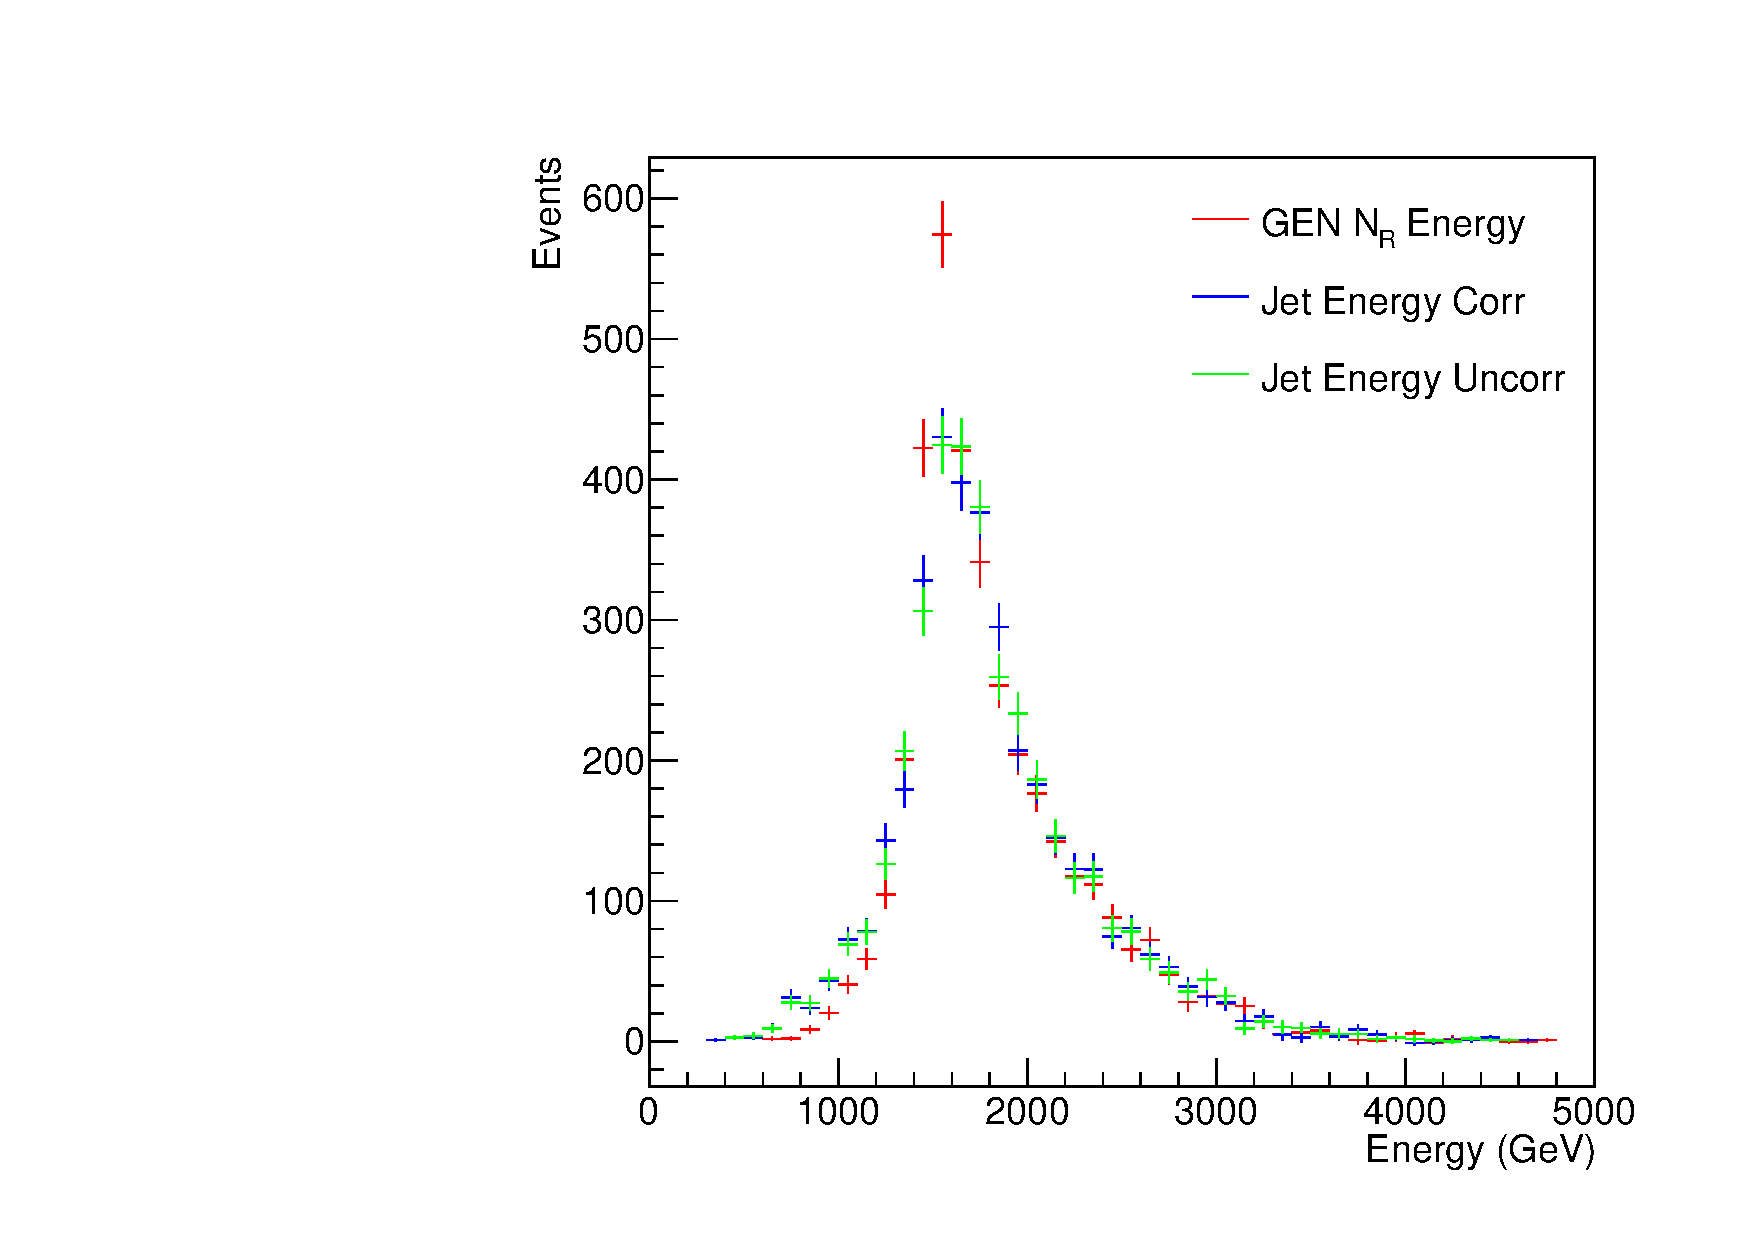
\includegraphics[width=\textwidth]{figures/JetEnergyVsNeutrinoEnergy_3000_400.pdf}
    \caption[
        %Short caption for the list of figures
       Reconstructed Jet Energy vs Generated Neutrino Energy.
    ]{
        % Full caption shown below the image
        The generated right-handed neutrino energy is compared to the corrected and uncorrected jet energy for the AK8 jet reconstructing the neutrino. 
    }
    % A label so you can \ref{fig:my_fig}. It is arbitrary; neither the 'fig:'
    % nor the fact that it has the same name as the pdf are required.
    \label{fig:jetEvsNRE}
\end{figure}

\subsection{Jet Mass}
In the boosted right-handed neutrino analysis case, the jet forming from the neutrino is expected to reconstruct with significant mass. With additional interactions occurring in the detector, the soft drop algorithm is used to mitigate wide-angle soft radiation in the jet contributing to its mass. With a jet of radius \ensuremath{R_0} with just two members, the soft drop procedure removes the softer constituent unless:

\subsection{Lepton Subjet Fraction}

\section{Muons}
\subsection{Reconstruction}
\subsection{Identification}
high-pt muons
\subsection{Momentum Corrections}
Rochester corrections and generalized-endpoint method

\section{Electrons}
\subsection{Reconstruction}
\subsection{Identification}
HEEPv7 and Loose
\subsection{Energy Corrections}

\section{HEM failure}
\label{sec:HEMfailure}
\CMS uses information from as many sub-detectors as possible to create reconstructed "particles".  Momentum and direction can be determined from the tracker, as well as the sign of the charge.  Charged particles and photons interact in \ECAL and long-lived charged and neutral hadrons interact with \HCAL. Muons typically rely on just the tracker and muon chambers, and are thus unaffected by the missing section of \HCAL.  Any hadronic activity entering this region then, suffers reduced precision.  While the process of showering in the detector is relatively well understood, the amount of energy that would be expected in the dark region of \HCAL must be extrapolated.  Electron identification also suffers, While there are many different properties that distinguish electrons in the detector, one key way they are distinguished from charged pions is that charged pions shower in \ECAL and \HCAL, electrons do not, as they are too light to travel this far.  The ratio of energy in \ECAL with the \HCAL sectors behind it is important to know, and impossible to extrapolate with \HCAL off.  Photons, on the other hand, are less affected, they offer up their entire energy in \ECAL and make a straight path through the tracker.  This makes them distinct from long lived neutral hadrons, which will shower in \HCAL and have no trace in the tracker.
